%%%%%%%%%%%%%%%%%%%%%%% file template.tex %%%%%%%%%%%%%%%%%%%%%%%%%
%
% This is a general template file for the LaTeX package SVJour3
% for Springer journals.          Springer Heidelberg 2010/09/16
%
% Copy it to a new file with a new name and use it as the basis
% for your article. Delete % signs as needed.
%
% This template includes a few options for different layouts and
% content for various journals. Please consult a previous issue of
% your journal as needed.
%
%%%%%%%%%%%%%%%%%%%%%%%%%%%%%%%%%%%%%%%%%%%%%%%%%%%%%%%%%%%%%%%%%%%


\RequirePackage{fix-cm}
%
%\documentclass{svjour3}                     % onecolumn (standard format)
%\documentclass[smallcondensed]{svjour3}     % onecolumn (ditto)
%
%\documentclass[smallextended]{svjour3}       % onecolumn (second format)
\documentclass[twocolumn]{svjour3}          % twocolumn
%
\smartqed  % flush right qed marks, e.g. at end of proof
%
\usepackage{graphicx}
\usepackage[spanish]{babel}
% \usepackage{mathptmx}      % use Times fonts if available on your TeX system
%
% insert here the call for the packages your document requires
%\usepackage{latexsym}
% etc.
%
% please place your own definitions here and don't use \def but
% \newcommand{}{}
%
% Insert the name of "your journal" with
\journalname{Autonomous Robots}
%
\begin{document}

\title{Jderobot open source framework for robotic, computer vision and home automation applications
%\thanks{Grants or other notes
%about the article that should go on the front page should be
%placed here. General acknowledgments should be placed at the end of the article.}
}
%\subtitle{Do you have a subtitle?\\ If so, write it here}

%\titlerunning{Short form of title}        % if too long for running head

\author{Jos\'e M. Ca\~nas \and David Lobato \and Roberto Calvo \and Julio Vega \and Eduardo Perdices \and Francisco Rivas}

%\authorrunning{Short form of author list} % if too long for running head

\institute{F. Author \at
              first address \\
              Tel.: +123-45-678910\\
              Fax: +123-45-678910\\
              \email{fauthor@example.com}           %  \\
%             \emph{Present address:} of F. Author  %  if needed
           \and
           S. Author \at
              second address
}

\date{Received: date / Accepted: date}
% The correct dates will be entered by the editor


\maketitle

\begin{abstract}
For a given robot most of its intelligence lies on its software, the way it coordinates its sensing and actuation capabilities. In the last years several frameworks have appeared that simplify and speed up the development of robot applications. They favor the code reuse and take benefits from modern software engineering techniques. This paper presents the open source robotics framework Jderobot, a distributed and component oriented platform. It uses explicit interfaces among components and ICE as communication middleware. It provides many tools for robot programming like a template for robot control components, visual HFSM creation, etc. Several examples of research and applications done with this framework are also described as experimental validation of it.
\keywords{Robot software \and Programming frameworks \and Code reuse}
% \PACS{PACS code1 \and PACS code2 \and more}
% \subclass{MSC code1 \and MSC code2 \and more}
\end{abstract}

\section{Introduction}
\label{intro}

%software importance
Most of robot intelligence lies on its software. Once the robot sensor and actuator devices are set, the robot behavior is fully caused by its software. There is no universally accepted way of programming robots. There are robots programmed in low level assembler and also in high level languages like C, C++ or Java. 

The importance of good programming practices has increased in the last years and also the interest in the robotics community on this topic. Several special issues of robotics journals (ARS Special Issue on Software Development and Integration in Robotics, 2006) and books on the topic \cite{brugali2007} have been published, specific workshops have been created inside ICRA and IROS, the Journal of Software Engineering for Robotics (www.joser.org) has appeared that promotes the synergy between Software Engineering and Robotics, and the Technical Committee for Software Engineering for Robotics and Automation inside the IEEE Robotics and Automation Society (TC-SOFT) has been created. Code reuse to avoid restarting from scratch for every new robot platforms and software integration are key issues in this topic. 

%Encapsulating robot capabilities in functions is a slippery issue as behaviors usually don't fit into the functional abstraction where the caller invokes the function and stops it flow of execution until receives the function response or output.

% software requirements in robotics
Compared with other computer science fields the development of robot applications exhibits some specific requirements. First, liveliness and real-time processing: software here has to take decisions with in a fast way, for instance in robot navigation or image processing. Second, robot software has to deal with multiple concurrent sources of activity, and so tends to be multitask. Third, computing power is usually spread along several connected computers, and so the robotic software may be distributed. Fourth, the robotic software typically deals with heterogeneous hardware. New sensor and actuator devices continually appears in the market and this makes maintenance and portability to new robots or devices more complex. Fifth, the robotic software usually includes a Graphical User Interface, mainly for debugging purposes. Sixth, the robotic software should be expansible for incremental addition of new functionality and code reuse. Seventh, the simulators are very useful in robotics software debugging.

% robotic frameworks 
Mobile robot programming has evolved significantly in recent years, and two approaches are currently found. In the classical approch the application programs for simple robots obtain readings from sensors and send commands to actuators by directly calling functions from the drivers provided by the seller. In last years several frameworks (SDKs) have appeared that simplify and speed up the development of robot applications, both from robotic companies and from research centers, both with closed and open source. They favor the portability of applications between different robots and promote code reuse.

First, they offer a simple and more abstract access to sensors and actuators than the operating systems of simple robots. Using the SDK hardware abstraction layer it deals with low level details accessing to sensors and actuators, releasing the robotics programmer from that complexity.
%For example, in a Pioneer with a laser rangefinder, the applications can obtain readings using ARIA or directly through a serial port. Using ARIA, one need only invoke a method and ARIA will take charge of refreshing the variables. Using the operating system directly, the application must request and periodically read the data from the laser through the serial port, and must identify the protocol of the device to compose and analyze the low level messages correctly. The abstract access is also offered for actuators.

Second, the SDK provides a software architecture for robot applications. It offers a particular way to organize code, allowing the handling of code complexity when the robot functionality increases. There are many options: calling to library functions, reading variables, invoking object methods, sending messages via the network to servers, etc.. Depending on the programming model the robot application can be considered an object collection, a set of modules talking through the network, an iterative process calling to functions, etc.

Third, usually the SDK includes simple libraries, tools and common use functionality blocks, such as robust techniques for perception or control, localization, safe local navigation, global navigation, social abilities, map construction, etc. This way SDKs shorten the development time and reduce the programming effort needed to code a robotic application as long as the programmer can build it by reusing the common functionality included in the SDK, keeping herself focused in the specific aspects of her application. The robot manufacturers sell them separately or include them as additional value with their own SDKs. For example, ERSP includes three packages in the basic architecture: one for interaction, one for navigation and another for vision. 

%% \begin{figure*}
%%   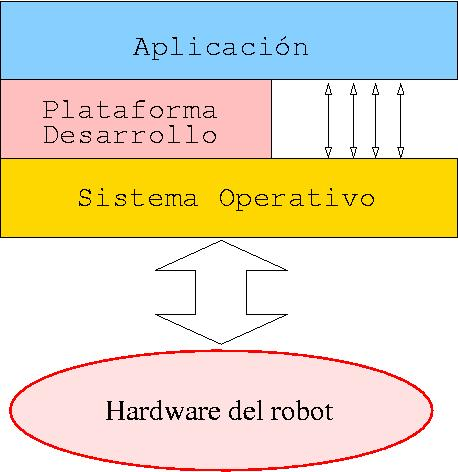
\includegraphics[width=7cm]{figs/programacion3.jpg}
%% \caption{Please write your figure caption here}
%% \label{fig:2}  
%% \end{figure*}

% our proposal
We present our open-source robotic software framework, named Jderobot, which is component oriented, uses ICE as communication middleware and includes several useful tools and libraries. Several sensor and actuator drivers have been programmed or reused from the open-source community. This framework has been widely used in our group for research and teaching for more than ten years. Jderobot has been designed for scenarios with sensors, actuators and intelligent software in between. The typical scenario is robotics, but also computer vision and home automation.

% open source
Why open-source in robotics? First, it provides independence on robot manufacturers and so it may support robots from different companies. Using open-source you are free to modify, debug, or improve the software, so the final software quality is high and does not depend on a single company debuggins speed. One strong motivation is also the feeling of contributing to the robotics community and to return the favor. We have extensively used open-source libraries and tools in our research (OpenCV, Gazebo, GTK, etc.). Research algorithms can be replicated easily and compared with standard tools. The tools must be open in order to trust in them.

% paper organization
This paper is organized as follows. The state of the art in robotic frameworks fills section \ref{sec:relatedworks}, where other platforms are briefly presented. Section \ref{sec:jderobot} fully explains the proposed platform, the ideas behind its design, the set of standardized interfaces and developed drivers, and the tools included to make the development of new applications easier. In section \ref{sec:applications} some successful examples using Jderobot are presented, both in research and in teaching. Final section summarizes the main conclusions and lessons learnt.

\section{Related works}
\label{sec:relatedworks}

Robotic frameworks can be grouped in two main paradigms, those tightly
coupled with a cognitive model in their designs and those designed
just from a pure engineering criteria. The first ones \textit{force}
the user to follow a set of rules in order to program certain robotic
behavior, while the second ones are just a collection of tools that
can flexibly be put together in several ways to accomplish the task.

%cognitive frameworks
Cognitive robotic frameworks were popular in the 90s and they were
strongly influenced by the AI, where planning was one of the main
keys. Indeed one of the strengths of such frameworks were their
planning modules built around a sensed reality. A good example of cognitive
frameworks was Saphira \cite{konolige98} based on a behaviourist
cognitive model. Some of its low-level functionality was rewritten as a
C++ library called ARIA \cite{aria} that it's still supplied with the
popular robotic platforms from MobileRobots/ActivMedia. Even though
the underliying cognitive model usually is a good practice guide for
programming robots, this hardwired coupling often leads the user to
problems difficult to solve when trying to do something the framework
isn't desing to do.

%current frameworks
Current robotic frameworks focus their designs on the requirements
that robotics applications need and let the user (the programmer) to
choose the organization that better fits with her specific
application. Main requirements driving the designs are: multi-tasking, distributed, easy to
use and code reusability. Another requirement, we believe it's a main
key, it's the open source code, that creates a synergy between the user
and the developer. 

%key achievements
Key achievements of modern frameworks are the hardware abstraction, hiding the complexity of accessing heterogeneous hardware (sensors and
actuators) under standard interfaces, the distributed capabilities
that allows to run complex systems spread over a network of computers,
the multi-platform and multi-language capabilities that enables the
user to run her software in multiple architectures, and the existence
of big communities of software that share code and ideas.

%open source
As said before, we believe that open source plays a mayor role in the
developement of modern robotic frameworks. Proof of this is the two most popular robotic
frameworks in the last years: Player/Stage
\cite{Gerkey03,collet05,vaughan2007} which has been the \textit{standard de
facto} in most of the last decade and ROS \cite{quigley09} which is
taking the place currently. As seen in other mayor software projects
as GNU/Linux kernel or the Apache web server, to name but a few, the
creation of communities that interact and share code and ideas, could
be a great benefict to the robotic community. Main examples of open
source modern frameworks are the aformentioned PlayerStage and
ROS. Another important example is ORCA \cite{brooks05,brooks07}. We
brefly describe them.

%%CARMEN \cite{montemerlo03}
There are other open source frameworks that have had some impact on current the state of the art, like CARMEN \cite{montemerlo03} by Carnegie Mellon or Miro \cite{Kraetzschmar02} by University of Ulm. Both use some component based approach to organize robotic software using IPC and CORBA, respectively to communicate their modules.

%Non-open source solutions
We can find non open source solutions as well, like Microsoft Robotics Studio or ERSP by Evolution Robotics. 

\subsection{Player/Stage}
Player/Stage framework provides the Player robot device server and the
Stage multiple robot simulator, plus several tools and libraries to support the
development of robotic applications. Player/Stage has been the most
popular framework in the last decade and it has a big community that
has create a great collection of drivers and algorithms around it. It has a platform independent implementation and it has support for the most common programming languages, like C/C++, Python, Java,...

Player provides a network interface to the robot hardware through a collection of standard
interfaces that provides a hardware abstraction layer. This standard interfaces are implemented by drivers, one
for each different hardware. This way a user only needs to know the
standard way to use, let say, a laser ranger and not every different
brand. Player exports its devices through a standard TCP network
connection  (other transport layers are available as well)
enabling the user to build distributed systems across a network of
computers. Even though, Player wasn't desinged as component based software, its architecture employs many component based
ideas. In addition to hardware drivers, Player has a collection of algorithms
like local navigation algorithms, vision related algorithms or
localization algorithms. 

Stage is a 2.5D multiple robot simulator that can provide its
simulated devices through a Player server. There's a big variety of
devices Stage can simulate, like laser ragers, robotic platforms and
cameras, to name a few.

The typical organization of a robotic application written in Player/Stage is one or more client programms subscribed to a Player server set to serve the robot hardware. Clients send and receive the data using the known interfaces. So, we can say Player/Stage has a centralized architecture, where Player server plays the main role. To run code on the server side, a user can write a driver that implements an interface, but this task it's usually a bit harder that the client side programms and some advanced knoledge of Player/Stage is required.

\subsection{ROS}
ROS is another important example of robotic frameworks. It was founded by Willow Garage as an open source initiative. Currently has a growing community
and its site hosts a great collection of hardware drivers, algorithms
and other tools. It is a multi platform and multi language framework.

Tha main idea behind ROS is a extremly easy to use hibrid (message passing and RPCs) middleware that allows to connect several components, implementing the robotic behavior, in a distributed fashion over a network of computers. Message passing of typed messages allows components to share information in a deoupled way, where you don't know which component send you a message, and viceversa, you don't know which component or components will receive your message. RPC mechanisms are available as well. Resources can be reached through a well defined naming policy.

The ROS core libraries implement the communication mechanisms and a set of tools to help with tasks as project management (cmake based), system
debugging and centralized logging. A set of official libraries implement standard messages (sensors, geometry, action,...), well known robotic algorithms for navigation or sensor analisys, and powerful tools as the rviz 3d visualization environment for robots. A simulation enviroment is provided through the Gazebo 3D simulator, that started as a part of the Player/Stage project, but now is supported by Willow Garage.

A typical application written in ROS is a collection of components interacting with each other (no server/client model) distributed among a network of computational nodes. Often a user can just use some of the components found in the ROS repositories, tweak some parameters and make them interact with his own coded components.

\subsection{ORCA}
Another important example is ORCA, a component based framework released several years before ROS. ORCA is multi platform and multi language as well. The aim of its developers was to increase the software reuse among the robotic community, so they create a component repository for robotics applications and they provide some of the needed \textit{glue} to connect them. In a previous version, they code the middleware that enabled components to communicate. Later they realized that programming a middleware was out of the range of their interests, besides being a complex and time consuming task, so they replaced it with the professional grade middleware Ice from ZeroC \cite{henning04} that allowed them to focus in the robotic problems. ORCA has play a mayor source of inspiration for the Jderobot framework and some of its core components are closely related to this framework.

As a component based framework, a typical application written in ORCA has an architecture similar to the one described for ROS.

\section{Jderobot platform}
\label{sec:jderobot}
%intro: ya se cuenta en subseccion ``some history''
%The Jderobot platform is the result of the knoledge adquired through
%the development of several projects. The root comes from the doctoral
%thesis \cite{canas02} where the underlying cognitive architecture JDE (acronym in Spanish for Dynamic
%Schema Hierarchy) is
%described. An initial implementation called \textit{jdec} was provided
%where the main idea of organizing the
%software in an intelligent way was developed. Through the years many
%applications have been developed, not only in 
%the robotics field, but in domotic and computer vision fields.

%main characteristics
The Jderobot platform is a component based framework that uses the powerful object oriented middleware Ice from ZeroC as \textit{glue} between its parts. This important design decission allows Jderobot to run in multiple platforms and to be programmed with the most common programming languages (all the languages supported by Ice indeed). Jderobot components can also be distributed over a network of computational nodes and by extension use all the mechanisms provided by Ice as secure communications, redundancy mechanisms or naming services. 

%The platform is supported by a community of developers and its code is open source, released under a GPLv3 licence. A user community is available at \textit{http://jderobot.org}, where users can find documentation, downloads and examples. %%ya se cuenta en seccion jderobot as opensource

%brief description of the underlaying cognitive architecture
The Jderobot platform was developed under the influence of the JDE cognitive architecture \cite{canas02,canas05e}. In early releases, the user was \textit{forced} to follow the main lines of JDE. Currently the underlaying conceptual architecture is just a good practices guide and the user can choose to follow it or not. Briefly, the main lines of the JDE cognitive architecture are as follows:

\begin{itemize}
\item Behavior = {perception} and {control}
\item Divide and conquer: behavior is fragmented is smaller parts called \textit{schemas}
\begin{itemize}
\item[-] Perceptive schemas elaborate estimuli
\item[-] Motor schemas generate control
\end{itemize}
\item A collection of schemas is organized as a dynamic hierarchy
\item Behaviorist aproach
\end{itemize}

The main unit is the schema. A schema is a continous and independent execution flow with some goal. Its activation state can be activated and deactivated at will, and its parameters can be modulated.

%component = schema
The definition of schema has big similarities with the definition of component (from a software enginiering point of view), and this is the main link between the Jderobot framework and the underlaying cognitive architecture. A behavior is fragmented in smaller parts (schemas) and then implemented as components.

\subsection{Software architecture design}
The first official release of Jderobot was 4.3. The core functionality was a collection of shared variables that represented the state of the sensors and actuators attached. A collection of schemas, implemented as a collection of threads, read and wrote these shared variables in order to achieve their goals. There wasn't a explicit API to write or read values from these variables, but just an agreement between writters and readers about the meaning of such variables. Some basic distributed mechanisms where implemented, bat mainly as ad-hoc solutions.

This design worked well for small projects, but as soon as we start implementing more complex systems some important drawbacks arose, like access sincronization, divergencies in the semantics of shared variables among schemas, or the poor distribution solution. All this feedback was very valuable and we chose to completely redesign the Jderobot framework, applying all the lessons learnt.

Following current trends in robotic software engineering we aim to design a framework with these mayor requirements:
\begin{itemize}
\item Component based
\item Multi-platform and multi-language support
\item Distributed
\item Strongly typed interfaces
\item Open source
\end{itemize}

%why Ice
Systems with some of these requirements are often hard to build. Because of this, we decided to find an existing middleware that coud cope with our requirements. The selection of Ice as the middleware for Jderobot was the most important design decission. This way we could use more efforts to design and program robotic related software and less to deal with problems already solved by Ice where we are no experts. Ice is the main building block of Jderobot.

%component based
The programming model is based on components. A typical Jderobot application is a set of components running concurrently, as different operating system processes. They communicate sharing messages between them, cooperating to achive the desired behavior. Components are the basic unit in Jderobot. A Jderobot component is usually implemented around the \textit{Ice::Application} class running on the main thread of a process, and optionally other service threads performing optional tasks. This main thread execute the component main task, that usually has the form of an iterative task running continously at a specific rate. This iterative task includes the communications task, that sends or receive data. This model is opposed to the one used in previous releases of Jderobot, where basic units were implemented using threads. It's straightforward to see that the use of processes as the basic unit will make easier the approact to the remaining design requirements.

%multi-platform & multi-language
Jderobot is able to interoperate between multiple platforms (Windows, GNU/Linux, MacOS, Android, ...) and it has support for multiple programming languages (C++,Python, Java, PHP,...), as Ice has support for main architectures and for most popular programming languages.

%distributed
Ice provides several communication mechanisms, from syncronous and asyncronous standard RPCs to subscription mechanisms, where multiple publishers and subscribers can interact. This allows Jderobot to provide a rich set of options to provide communication between its components, allowing those components to be distributed over a network of computers. Moreover, Ice has several tools that allows to provide redundant and/or failsafe services.

%interfaces
Jderobot components communicate through interfaces. They define the minimum communication unit between components. Jderobot components implements these interfaces to provide functionality and use them to use the functionality from other components. Interfaces are defined with \textit{slice}, the interface definition language used by Ice, that describe their data structures and operations. This slice definitions are then used to generate code for the desired programming languages.

%open source & software reuse
In addition to Ice, Jderobot uses other open source libraries like OpenCV, Gearbox, OpenGL, Player/Stage or GSL, to name but a few, for the same reasons exposed above: we want to focus our efforts to design and program robotic related software. In return, we release all our code as open source and we encourage our community to follow these ideas.

%gui & config files
Other two minor requirements were present in the design process. First, Graphical user interfaces are especially useful for debugging purpouses or for human interaction. Previous releases of Jderobot needed ad-hoc approches because of the multi-threaded design, some wrappers where needed to make the share access to the screen easier. Nowadays, Jderobot doesn't make any special assumption on this subject, each component is a separate process, the user must choose the approach that better fits in each context. Some guidelines and examples are provided though, though design patters as MVC or implementations using popular graphic frameworks as GTK+. A Jderobot component usually will run a service thread with the graphical user interface computations. Second, schemas ara parametrized and its implementation counterpart requires any means to get this parameters. A simple approach is to use configuration files. Ice has native support for parsing simple text files with a format closely related to Java property files. Using this files components can get their specific parameters or the location of resources (files, other components,...). Ice provides a parameter server that could be used as a central configuration repository.

\subsection{Interfaces and drivers}

Beyond previous design principles, the Jderobot framework includes several components that manage different sensors and actuators and provide the applications with standard interfaces for accessing to those devices. Using ICE the access can be local or remote from a different computer. There is no one-to-one relationship between components and interfaces. One driver component may offer several interfaces at the same time, and the same interface may be implemented by several drivers.

% interfaces
There are interfaces for laser devices (laser), for Pioneer base control (motors), for RGB-Depth sensors like kinect, pantilt units (pose3Dmotors, pose3Dencoders), for image sources (camera interface), for home automation devices (x10), etc.. These interfaces together draw a Hardware Abstraction Layer to be used from the application code. 

Some interfaces are offered for different robots, favoring the applications portability. For instance, the \texttt{motor} interface includes translation velocity (V), rotation velocity (W) and side velocity (L). It is supported by the driver used with the Pioneer wheeled robot and by the driver used with the legged Nao robot.

The same interfaces are also provided by drivers connected to the real devices and drivers connected to simulators like Gazebo, allowing the applications to run exactly the same on real robot than on simulator. 

% driver component
PlayerServer, GazeboServer for Gazebo Simulator , NaoServer, KinectServer, OpenNIServer, giraffeServer, PTU, Hokuyo, Wiimote, CameraServer.

\subsubsection{CameraServer}


\subsubsection{PlayerServer}

\subsubsection{GazeboServer}
\label{subsec:gazeboserver}

Jderobot integrates two servers, named PlayerServer and GazeboServer, which are used to communicate Player and Gazebo simulators (\cite{koening2004}) with other software components in the Jderobot platform. It's possible to retrieve information from several sensor devices, such us: laser, encoders, motors, cameras or sonars. And it also supports one or more cameras with their pantilt units (SonyVid30 model).

\subsubsection{NaoServer}

Nao robots include an internal Framework called ''Naoqi'', which provides an API to command and read the robot's motors and sensors. This API can't be directly deployed by other Jderobot components, since its functions are ad-hoc designed to Nao robots.

We have created an application called NaoServer, that runs inside the Nao robots and provides several standard ICE interfaces which may be used by other Jderobot components. NaoServer receives through ICE interfaces commands from other components and translates these commands to Naoqi.

\subsubsection{KinectServer and openniServer}

Kinect is one of the latest generation device more used in the last months. That is why jderobot icludes two drivers to support this device and allows to access to all the information that it provides. Through Jderobot you can access to color, depth and IR values, and also to the tilt motor device and it leds.

These two kinect servers are standardized to provide RGB and depth images as conventional cameras, so these sensors can be used with any jderobot application that uses the standard interface for cameras.
To work with the cloud of points obtained from the kinect  depth sensor jderobot  is supported by Point Cloud Library (PCL). This framework includes a large number of features for point cloud processing such as filters, model fitting and segmentation. 

Both servers use the OpenNi driver developed by PrimeSense. OpenNi is a framework aimed to develop applications that use natural interaction by offering access to low-level devices and also Middleware functions for visual tracking using computer vision. 

KinectServer accesses to the device through the openni\_grabber that PCL includes. This grabber is a very simplified version of the PrimeSense framework and only supports the RGB camera and depth sensor.

To access the device, openniServer uses directly the OpenNi framework. This driver supports all the kinect components (tilt motor, leds, RGB/IR camera and depth sensor). In this way it keep all the functionality of the middleware that offers subjects detection and tracking, user position, hands tracking...

Although the servers access information in a different way, both offer information using the same ICE interfaces so both components are completely compatible. 

\subsubsection{X10Server}

Home automation.

+ wiimote.

\subsubsection{GiraffeServer}

\subsection{Tools and libraries}

\subsubsection{FuzzyLib}

Fuzzylib is a library to design and program fuzzy controllers. The control rules are written in a file with simple rules like: IF ( left\_obstacle\_distance = small ) AND ( translation\_speed = high ) THEN ( rotation\_speed = right\_high ). 
%AND and OR fuzzy operators are supported in rules. 
The fuzzy labels and variables are also described in such file following a trapezoidal pattern and they are attached in the software to input and output variables of the control program. The controller automatically fuzzyfies the input variables, apply the rules and defuzzifies the output following a Center of Mass combination.

\subsubsection{VisionLib}
\label{subsec:visionlib}

Mathematical functions used on visual perception purposes can be found on this vision library. It contains computer vision research code initially developed to support the RobotVision project. It has since been expanded to provide a range of software infrastructure for computer vision, geometry models and images mechanisms. The library builds on top of the OpenCV Computer Vision Library\footnote{http://opencv.willowgarage.com/wiki} and the GNU Scientific Library\footnote{http://www.gnu.org/software/gsl} (GSL).

The structure of this library is as follows:
\begin{itemize} 
\item \textit{Cvfast} class provides the functionality of the Image Corner Detector called FAST.
\item \textit{Geometry} class contains implementations of different visual geometry purposes: intersections, distances, vector operations, segments operations, etcetera.
\item \textit{Image} class includes operations such as: Multiply Fast Fourier Transform or Get Segments.
\item \textit{LinesDetection} class provides the implementation of an Image Border Detector based on an article by A. Solis (\cite{solis09}).
\item \textit{Structs.h} header contains different useful structs for computer vision purposes.
\end{itemize}

\subsubsection{Progeo}
\label{subsec:progeo}

In order to facilitate the use of pin-hole calibrated cameras (see Figure \ref{fig:pinholemodel}) as well as certain geometry functions used for the purposes of performing 2D and 3D images calculations (such as 2D to 3D transformation and viceversa), Jderobot provides a library called ProGeo.

\begin{figure}[h!]
  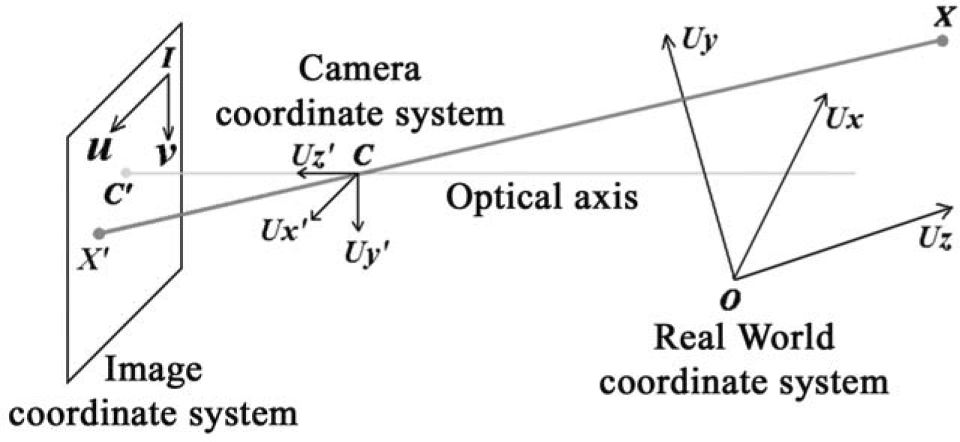
\includegraphics[width=8.5cm]{figs/pinholemodel.png}
\caption{Pin-hole model of a camera.}
\label{fig:pinholemodel}
\end{figure}

Some of the data types provided by this library are: \textit{HPoint2D} (to store a 2D point that usually belongs to the image plane), \textit{HPoint3D} (data point structure that represents a point in the 3D space) or \textit{TPinholeCamera} (pin-hole camera model defined by its extrinsics and intrinsics parameters).

And some of the functions which can be found are: \textit{project} (to project a 3D point on to the 2D image planer) and \textit{backproject} (to obtain the projection line that connects the camera with the focus and the 3D ray which is projected in a pixel of the image plane).

\subsubsection{Colorspaces}: espacios de color para imágenes

\subsubsection{Control template}

A basic component is included as a template for reactive controllers. It has two different threads, one for computation and a second one for visualization. Both threads run in continuous iterations at a given configurable rate, not more to avoid excesive CPU consumption. In case of heavy computations or overload of the CPU the system degrades gracefully running at the highest rate possible. This basic component has also been used for perceptive, localization and image processing algorithms.

\subsubsection{VisualHFSM}

There are many ways to organize the control and perception code on board a mobile robot. One succesful way are the Finite State Machines. With them the robot behavior is defined by a set of states, each of which performs a particular task. The robot can switch from one state to another through transitions (conditions of stay or change), depending on certain events or conditions, internal or external. A tool has been developed and included in Jderobot to graphically design hierarchies of FSM, insert the specific code of states and transitions, and automatically generate the component source code in C++.

\begin{figure}[h!]
  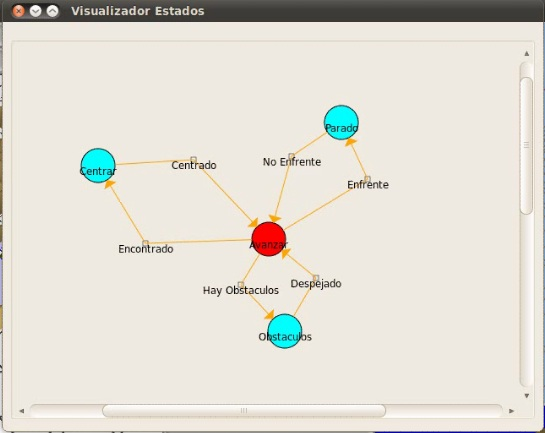
\includegraphics[width=8.5cm]{figs/ratonGatoAutoEjec.jpg}
\caption{Tool for visual HFSM design}
\label{fig:visualHFSM}
\end{figure}

\subsubsection{Calibrator}

The calibrator tool is used to calibrate external (position and orientation) and internal parameters (focal distance, optical center...) of any camera. It allows a manual calibration where the user provides a 3D description of the camera surroundings, the calibrator draws what the image should be with a certain parameter set over the really observed image. The user then modify parameters until finds a correct matching (Figure \ref{fig:calibrator}). It also includes a fully automatic calibration based on DLT and a 3D pattern. It generates a file with the camera calibration parameter values and it is fully integrated with progeo library.

\begin{figure}[h!]
  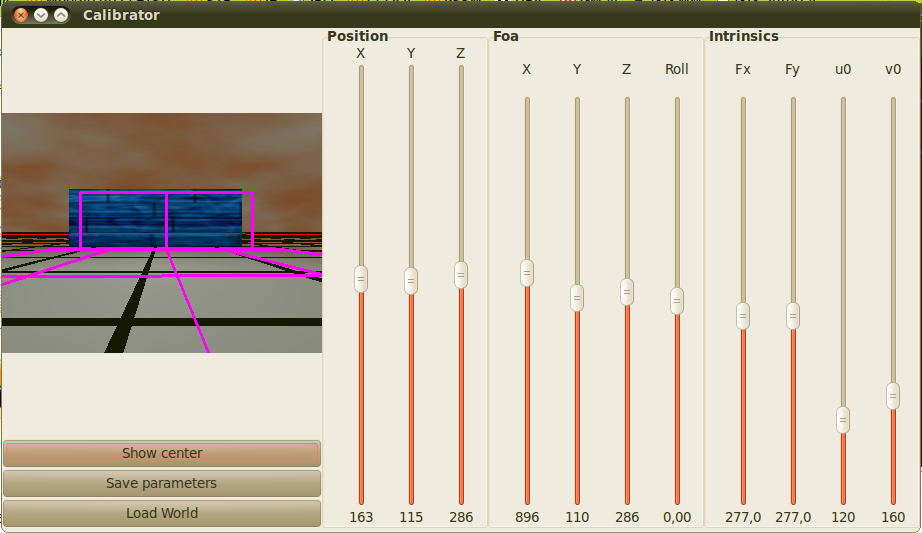
\includegraphics[width=8.5cm]{figs/calibratorGUI.png}
\caption{Calibrator in manual mode}
\label{fig:calibrator}
\end{figure}

\subsubsection{ColorTuner}

The colorTuner tool is used to adjust color filter in different colorspaces, like HSV, YUV, RGB, etc. For instance, the HS color disc is shown (Figure \ref{fig:colortuner}) and the color filter current thresholds are also displayed as a sector. It can be easily modified there, using sliders or clicking in sample pixels in current image.

\begin{figure}[h!]
  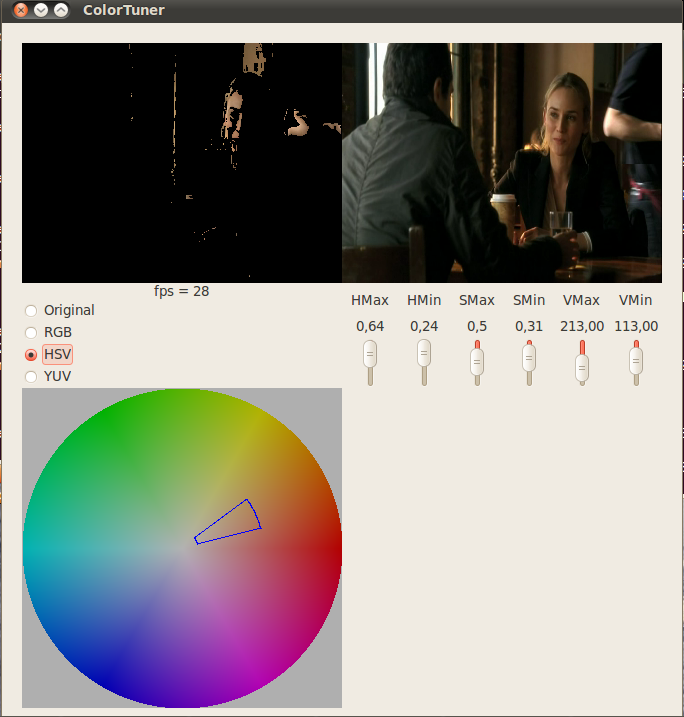
\includegraphics[width=8.5cm]{figs/colorTunerHSV.png}
\caption{ColorTuner tool for adjusting HSV color filters}
\label{fig:colortuner}
\end{figure}


\subsubsection{Recorder and replayer}

When we use real robots, one of the greatest difficulties is repeating experiments with the same conditions, whether we want to compare different algorithms or to test several features of the same algorithm. It's almost impossible to reproduce the same environment conditions, since robot hardware behaves diversely, light conditions change if we use cameras, people or objects move or are located in different places, etc.

To avoid all these matters, we have designed a new tool which records the current devices status and reproduces them whenever we want to. There are two components involved in this tool, the first one is the so-called ''recorder'', it saves in a file the status of all the devices of the robot, such as odometry, laser measures, image cameras, etc; we can configure which devices we want to track when we executes the components and it works with simulators, real Nao robots and real Pioneer robots.

The second components is the ''replayer'' component, it reads the file saved by the ''recorder'' component and provides the same ICE interfaces that would provide the real devices. Thus, when an algorithm gets the current devices status, it can't tell if it's obtaining the current devices measures in real time or pre-recorded data.

This tools has been widely used to perform experiments with real robots, to try different parameters and improve our algorithms.

Genérico, configurable qué sensores se graban y/o reproducen.

\subsubsection{Android mobileTeleoperator}

Android operating system is increasing its market share every day, both with smartphones and tables. Once you develop an application for this platform, it may be used by students, other researchers or even companies. 

We have created an application called ''Mobile Teleoperator'' to teleoperate either a Pioneer robot with playerserver or a Nao Robot with BICA architecture. Connection among the mobile device and the robots is made through ICE, the same way we do when we use a standard computer, so we don't need to change anything in Jderobot architecture.

There are three ways to teleoperate the robots:
- Arrows: After pressing a button, it sends the command to the robot and the robot keeps his behavior until the stop button is pressed.
- Joystick: While a button is pressed, it send the command to the robot, but if the button is released it sends a stop command automatically.
- Accelerometer: It uses the mobile accelerometers to command the robot depending on our device orientation. To use this behavior you must keep a ''safety'' button pressed, this button is used to calibrate the accelerometers when it is pressed the first time and to send a stop command automatically once this button is released.

Mobile teleoperator has been used to create demonstrations and to let people who are not used to control robot to teleoperate robots in a easy way.

\subsubsection{KinectViewer}

KinectViewer is able to connect to one of the kinects servers described  in the drivers section. Basically is a graphical interface witch represents the kinect information in two different ways: it can display directly the images (RGB and DEPTH) that it gets on streaming from the server or it can reconstruct an scene from the point cloud in an OpenGL world. This component also includes some of the 3D tools that jderobot provides to improve the data analysis. 


\section{Research, teaching and applications}
\label{sec:applications}

Once the main software components and design principles of Jderobot have been presented in previous section, in this one we describe some of the succesful research and applications done with it, that somehow probe its usefullness. Applications with sensors and actuators.

\subsection{Teaching robotics with Jderobot}

Special Jderobot component, such as Introrob, has been developed for students, in which a number of pre-programmed instructions are used to let students construct their own applications.

Such an approach eliminates the need to know a lot about gears, motors, using sensors, calibration and allows students to have a working robot within little over an hour. And then, a migration path from this very simple starting level to an environment where more skills are required. The best way is to start with a simple level and have a programming environment, such as Jderobot, that supports working from the very simple to a slightly more advanced level.

\begin{figure}[h!]
  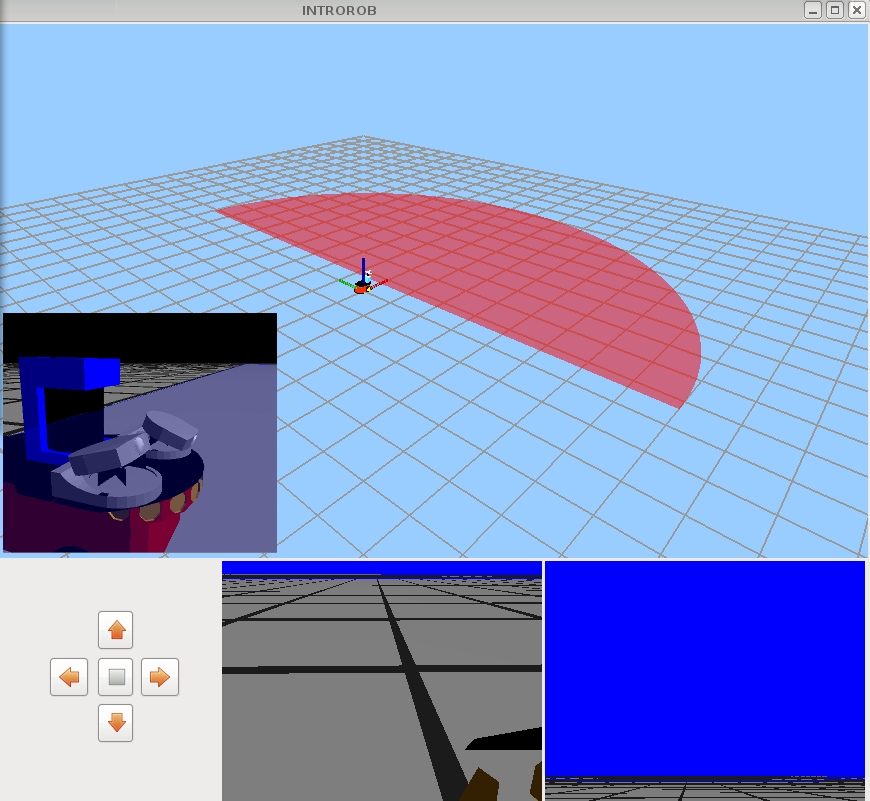
\includegraphics[width=8.5cm]{figs/introrob.jpg}
\caption{Introrob component Graphical interface.}
\label{fig:introrob}
\end{figure}

Having an integrated simulator is very important, so the students may quickly test their experiments without the need for a robot for every student. Such an environment is provided by The Player Project\footnote{http://playerstage.sourceforge.net/index.html} (see Section {subsec:gazeboserver}). This Open Source software is capable of simulating a population of robots, sensors and objects, but does so in a three-dimensional world.

\subsection{Robot navigation}

Obstacle avoidance is one of the key issues to successful applications of mobile robot systems. All mobile robots feature some kind of collision avoidance. It needs to steer the robot around the obstacle and proceed toward the original target.

We have implemented two famous navigation algorithms: VFF, as a obstacle avoidance or local path planning mechanism; and GPP, as a global path planner algorithm.

The Virtual Force Field (VFF) method is our earlier real-time obstacle avoidance method for our running robots. This technique allows for fast, continuous, and smooth motion of the controlled vehicle among unexpected obstacles, and does not require the vehicle to stop in front of obstacles.

On the other hand, when a trap-situation is flagged, the robot slows down (and may come to a complete halt),
while the VFF algorithm is temporarily suspended. The GPP algotithm is then invoked to plan a new path based on the available information in the gradient field that represents the optimal (lowest-cost) path to the goal at every point in the workspace (see Figure {fig:gppNav}).

\begin{figure}[h!]
  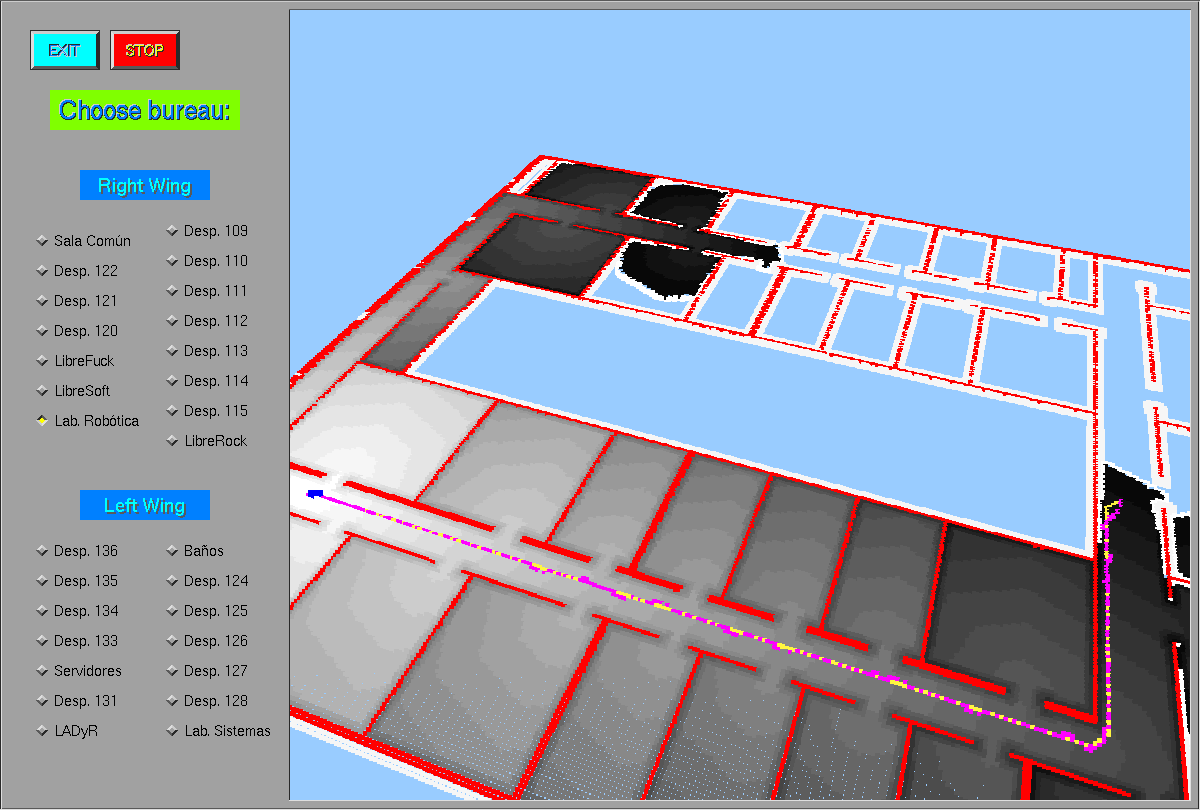
\includegraphics[width=8.5cm]{figs/gppNav.png}
\caption{Robot navigation using GPP and VFF algorithms.}
\label{fig:gppNav}
\end{figure}

Both techniques, VFF and GPP, have been implemented under Jderobot and extensively tested on Player-Stage and Gazebo simulators and on-board an ActivMedia Pioneer mobile robot, equipped with a ring of 24 ultrasonic sensors, and also using laser sensors, such as Hokuyo or Sick laser.

Follow person \cite{canas05d}.

\subsection{Evolutionary localization}

Self-localization is at the moment one of the most important challenges in robotics. Using robot sensors, such as cameras, laser sensors or ultrasonic sensors, our robot must be able to calculate its own localization inside an environment. Once the robot knows its position, it can adapt its behavior depending on where it is located. 
 
However, robot self-localization has proven to be one the most complex task on mobile robots, since they must face unknown situations, such as occlusions, or being located inside a dynamic environment.

With Jderobot, we have designed and implemented an evolutionary localization algorithm, a type of meta-heuristic optimization algorithm that is inspired by the biological evolution. In this kind of algorithms, candidate solutions evolve over time using genetic operators, such as mutation or crossover. 

The algorithm keeps several candidate solutions competing among each other in different positions. Thus, the evolutionary algorithm is able to handle several solutions at the same time, which is of great advantage when robots are located in symmetric environments.  

\subsection{MonoSLAM}

Monocular Simultaneous Localization And Mapping (MonoSLAM) is a type of localization first presented by Andrew J. Davison in 2003 (ref). MonoSLAM is able to construct a point-based map of the environment with a single camera, and localizates the camera inside this environment in real time.

We have developed our own MonoSLAM approach, based on Davison work, obtaining images from real cameras and simulators. We have implemented the point-based approach designed by Andrew Davison and afterwards we have designed our own implementations based on points and lines.

This type of localization is more accurate than classical localization methods and is very useful when robot odometry is not available or is not reliable. On the other hand, it is not able to handle occlusions and needs a faster frame rate.

\subsection{Visual memory}

The goal of our visual memory is to do a visual tracking of the various basic objects in the scene surrounding the robot. It must detect new objects, track them updating its relative position to the robot and remove them from the memory once they have disappeared.

The first stage of the system is a 2D analysis, in which 2D segments in the current image are detected using the Solis algorithm \cite{solis09} (see Section \label{subsec:visionlib}). Then the system puts these objects in 3D space according to the \textit{ground-hypothesis}, assuming they all are flat on the floor, and stores them in memory maybe merging with already existing 3D segments. 

\begin{figure}[h!]
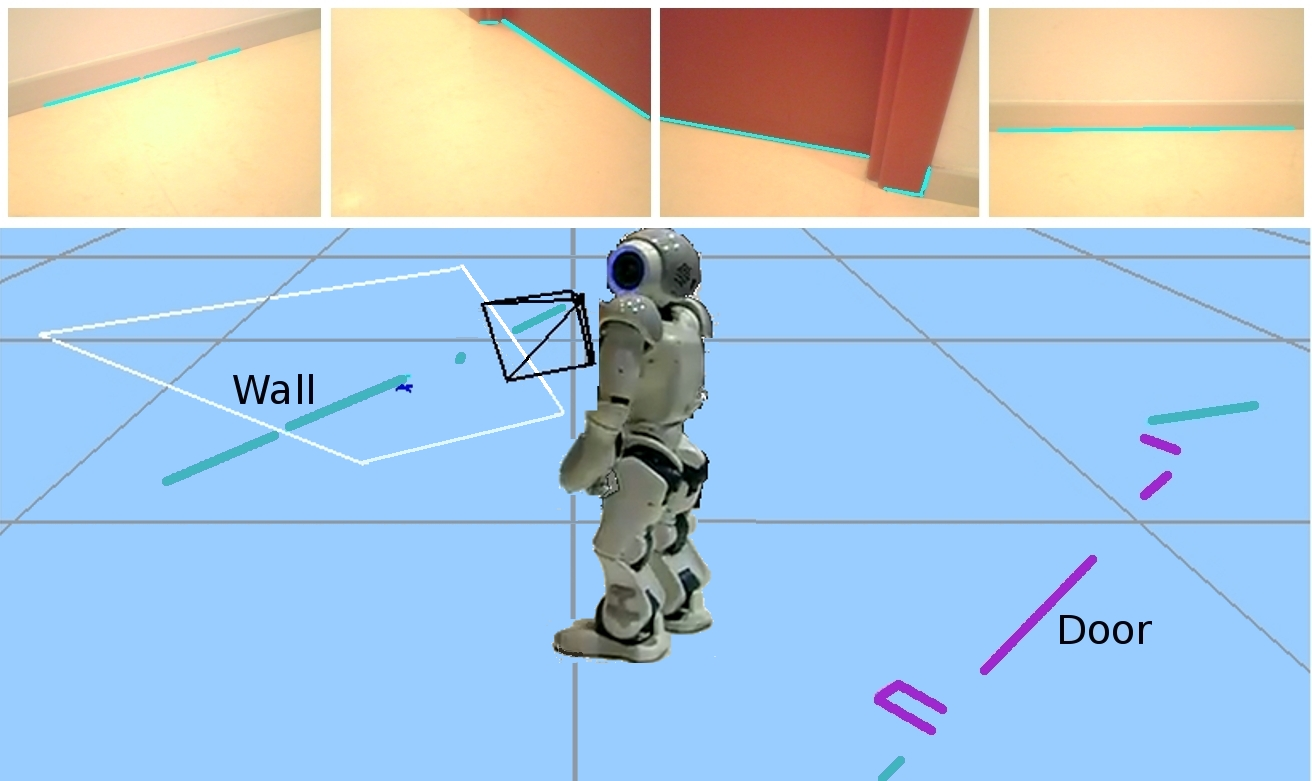
\includegraphics[width=8.5cm]{figs/experimentoReal.jpg}
\caption{Visual memory with 3D segments coming from four images of robot surroundings}
\label{fig:memory}
\end{figure}

Each 3D visible object already stored in memory is projected on the current image plane (using Progeo, see Section \label{subsec:progeo}. The system refutes/corroborates such predicted segments, comparing them with those extracted from current image. This comparison leads to three sets of segments. First, in case of matching the features of the stored 3D segment are updated taking into account the new observation. Second, if a segment is identified in the current image but does not match any prediction, the system creates a new one in 3D. Before inclusion in the 3D memory some post-processing is needed to avoid duplicates due to noise in the images, for instance comparing the relative position between segments, as well as its orientation and proximity. And third, for predicted segments not really observed in current image their quality goes down and eventually will be removed from memory.

\subsection{Surveillance}

Surveillance is a final application created using jderobot
framework. The goal of this application is built a surveillance
distributed system that can be controlled using an smartphone
device. Thanks to jderobot framework it is possible simplify the design
and development of this kind of complex applications.

The system consists in some webcams and pc scattered around the house
to watch over and detect any intruders or warning situations. Also, the
system can be controlled using an intelligent mobile (smartphone). As
you can see in the figure~\ref{fig:surveillance1} each important
feature of the system is implemented as a jderobot components. For each
webcam in the system it is mandatory have an instance of \emph{Recorder} and
\emph{CameraServer} components. The \emph{Recorder} component is
responsible for recording the video streaming in the hard disk. The
\emph{RecordingManager} component makes the configuration to
{Recorders} component and decides when and how a recording is
made. The \emph{CameraServer} component is a core component of
jderobot framework an is responsible for provide the video streaming as
RTSP format or image format to analyze movement in the scene. The \emph{Motion
  Detector} component make a movement detection analysis of the
scene. If a movement is detected by \emph{Motion Detector} component, it
sends a message to \emph{Surveillance} component that has all the logic of
the security system. The \emph{Surveillance} component is the responsible to
enable the \emph{Recording Manager} component and send messages to
start a recording when a movement is detected in the scene. Last, the
\emph{SecurityApp} component executes in an Android device and
exchanges information with \emph{RecordingManager} and
\emph{CameraServer} to show recordings, alarms or video streaming live.

\begin{figure*}
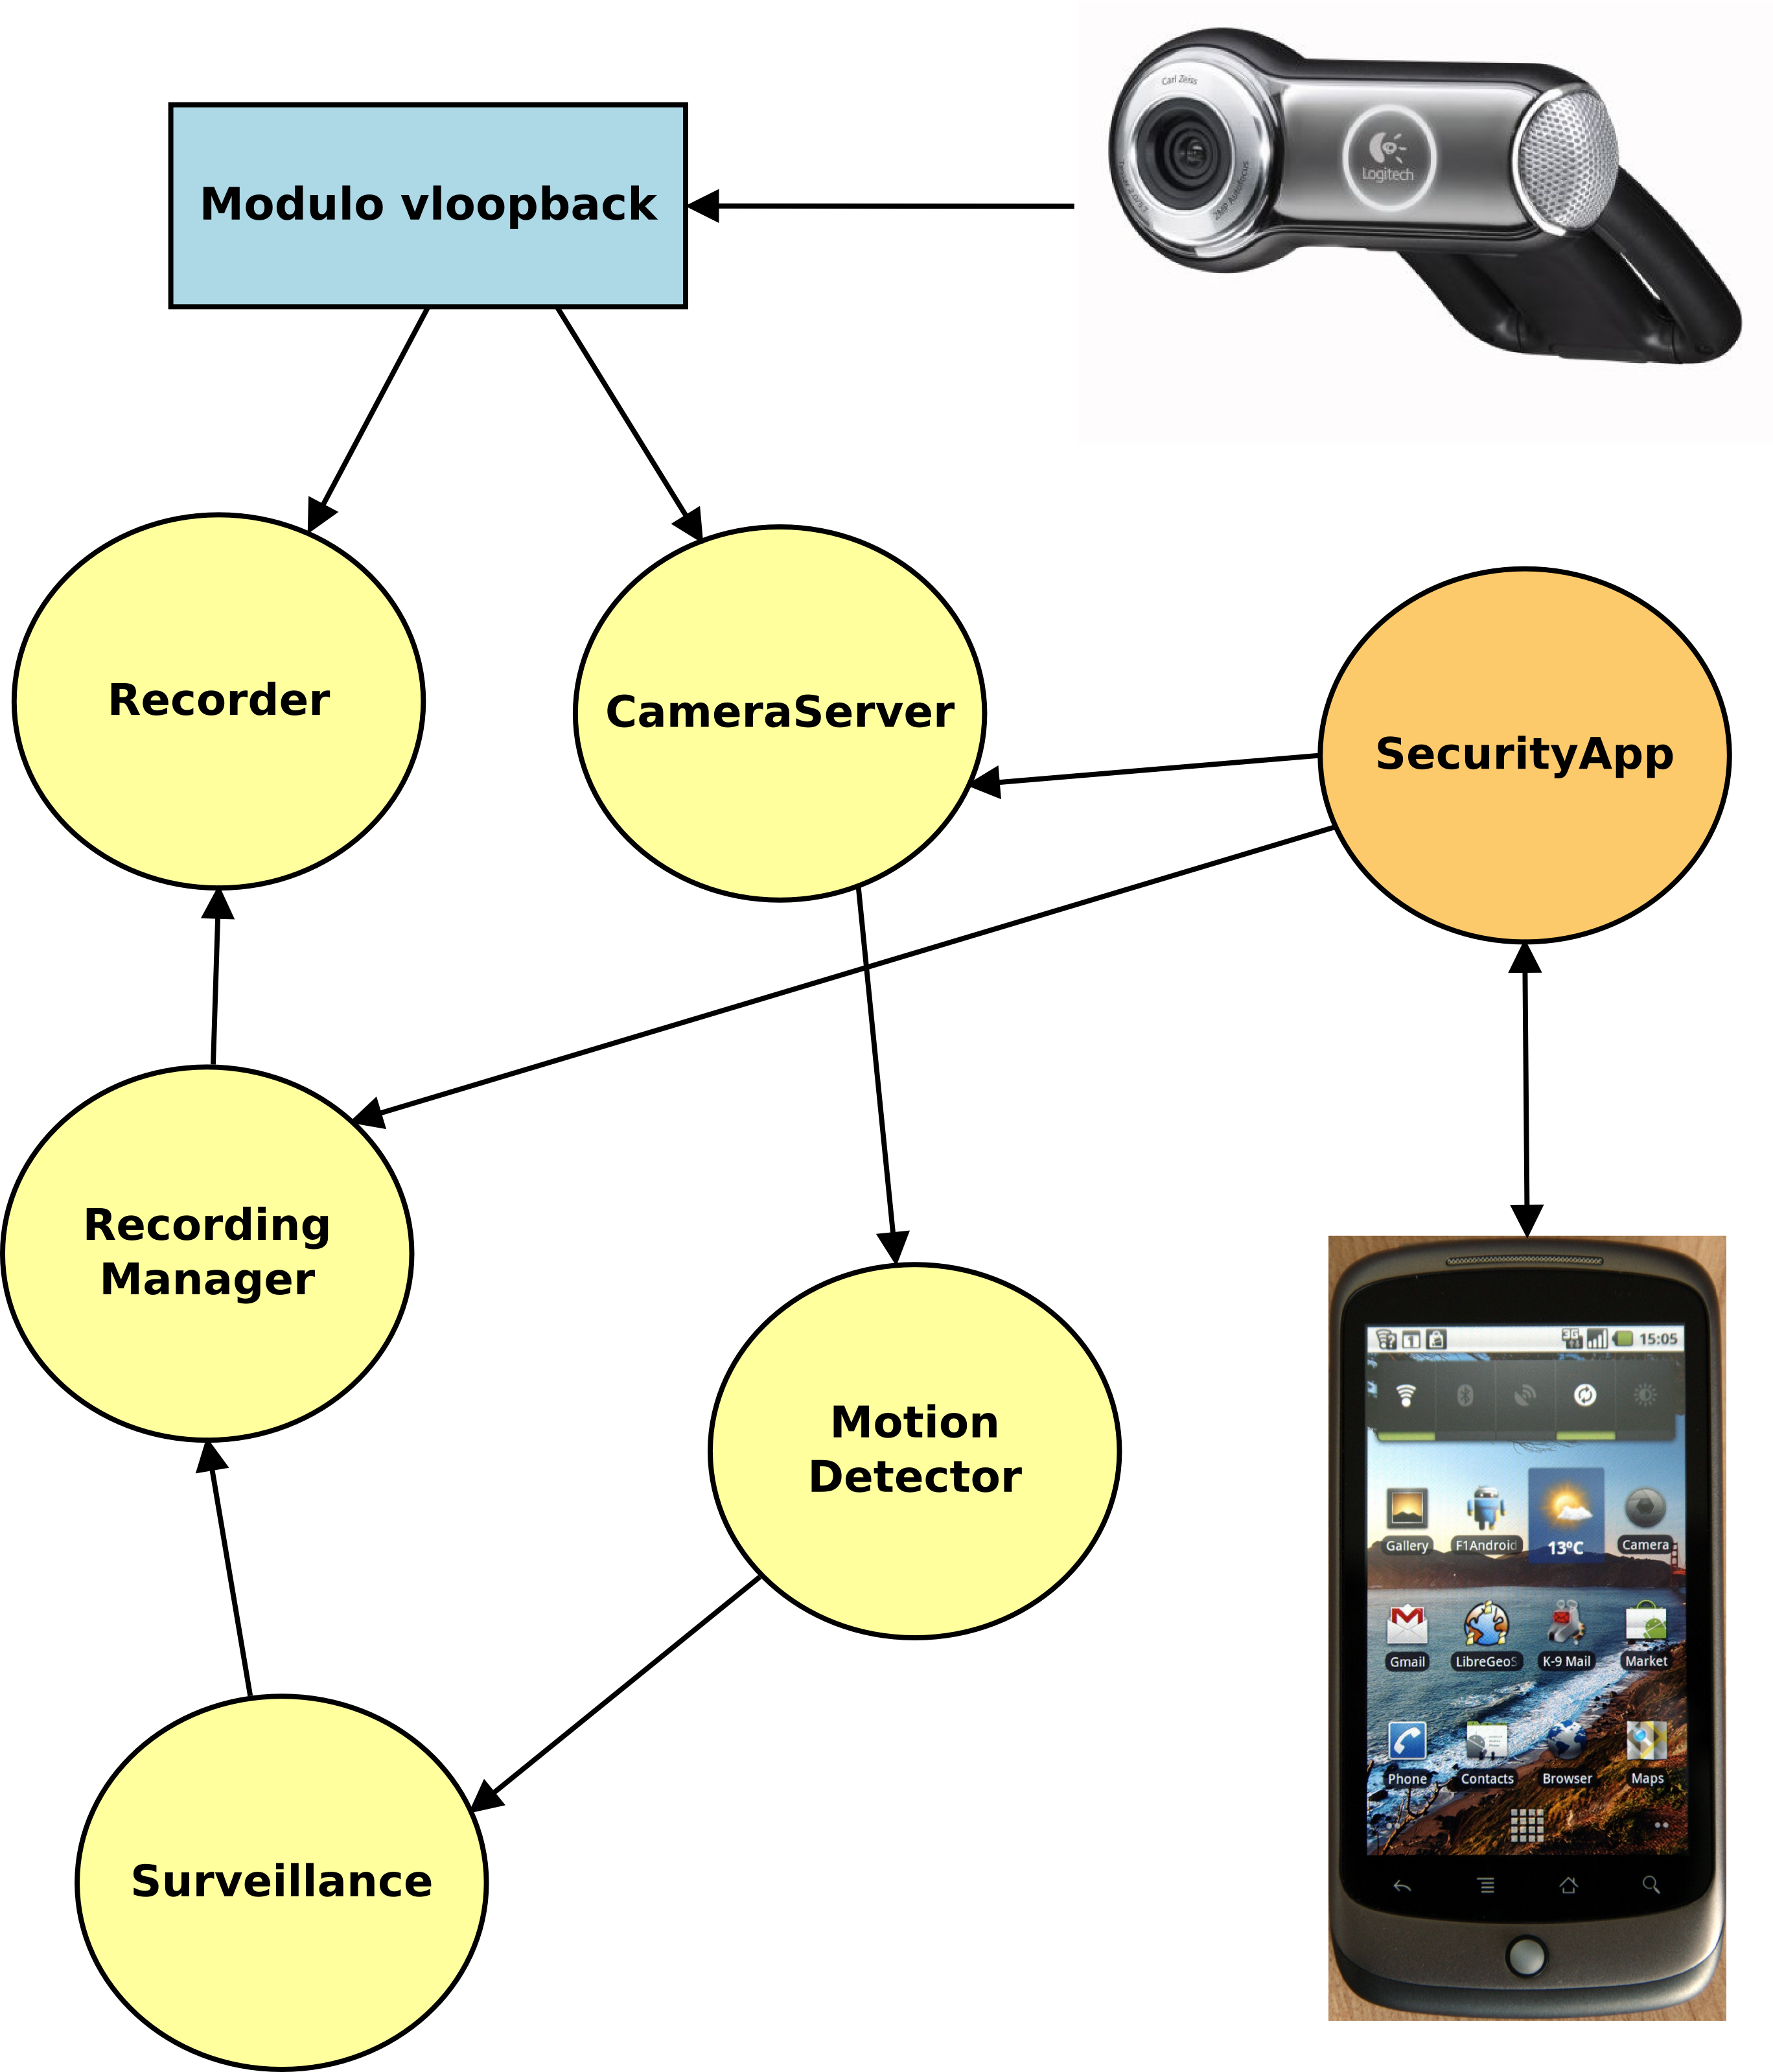
\includegraphics[width=6cm]{figs/surveillance-img1.png}
\caption{Global schema using jderobot components}
\label{fig:surveillance1}
\end{figure*}

The mobile application is very simple thanks to the abstraction of the
jderobot components because you do not spend time in communication
protocolos and other complex task. You only have to worry about the
functionality of the surveillance application. For example, you can
see in the figure~\ref{fig:surveillance2} the list of alarms that the
\emph{Recording Manager} component have stored. Also, it is possible
see the recordings associated with the alarms. The \emph{CameraServer}
component provides a video streaming live of the system webcams. You
can see in the figure~\ref{fig:surveillance3} how it is possible show
two video streamings live of the same room.

\begin{figure*}
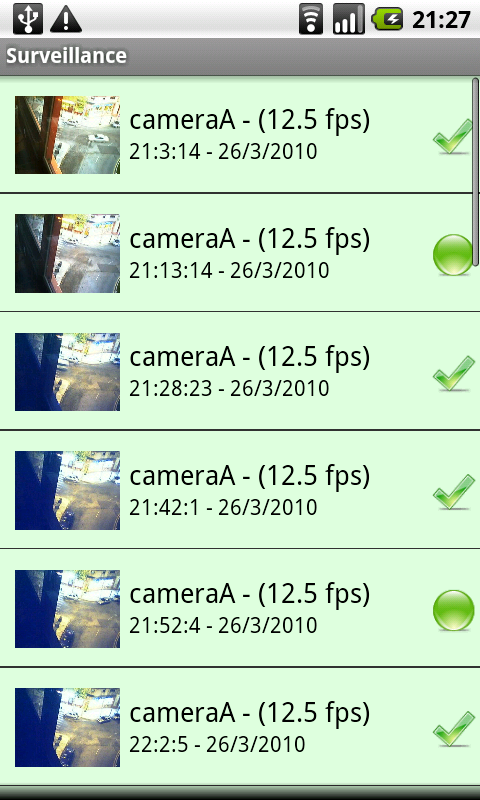
\includegraphics[width=6cm]{figs/surveillance-android.png}
\caption{Alarms list in the smartphone}
\label{fig:surveillance2}
\end{figure*}

\begin{figure*}
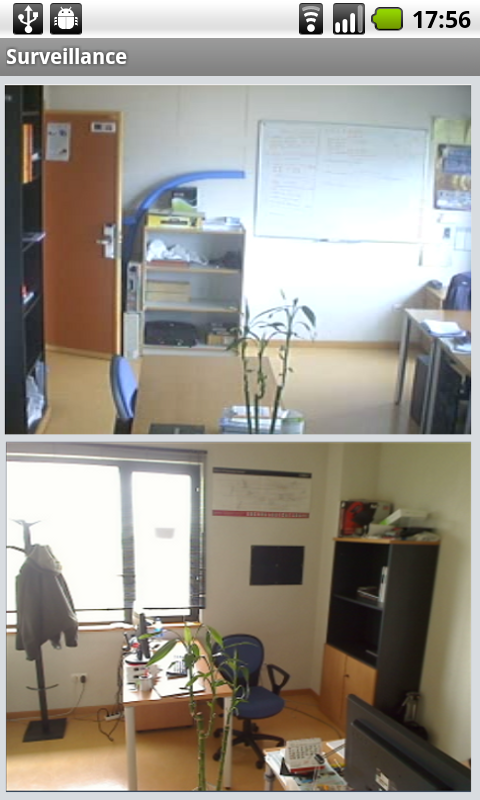
\includegraphics[width=6cm]{figs/surveillance-streaming2-recording.png}
\caption{Two video streaming of a room}
\label{fig:surveillance3}
\end{figure*}


\subsection{ElderCare}
Eldercare is a telecare-oriented application for elderly people living alone. The system is able to detect falls autonomously using only conventional cameras. Once a fall is detected the system automatically sends an alert to indicated medical personnel so that significantly reduces the waiting time in assistance occur.

The system does not require any action by the patient, do not need to wear any device over or any type of special  garment. It is a fully autonomous and non-intrusive system.

Eldercare can handle all alarms on a mobile phone. When a fall is detected, Eldercare can notify us the situation on a mobile phone and even allows us to watch the scene in real time through streaming images.

A new advance in the latest versions of eldercare is that the system has been complemented using Kinects devices, these devices are able to work as conventional cameras but have the main advantage of the on-board depth sensor. These devices work perfectly even without light, so the subject would be monitored in virtually any situation. 

\section{Jderobot as open-source project}

Jderobot project has a web page (jderobot.org) where the framework source code can be downloaded and its documentation accessed. The official manual is there in a MediaWiki. We prefer this web manual better than classic static documents, as the web manual update is agile and can be easily done by users themselves. We use a svn repository, trac for bug tracking, a blog and one mailing list for developers an users.

\subsection{Some history}

The Jderobot project started at 2002 in a PhD thesis, as the software implementation of a cognitive architecture to develop autonomous behaviors in robots \cite{canas02,canas05e}. It provided access to robot camera, encoders, sonar sensors and motors using sockets between some drivers and the (maybe remote) control application. The application was divided in \textit{schemas} that were implemented as concurrent threads in C language and organized as hierarchy. Its development was opened to a group of students. Several alternatives and expansions have been programmed since then \cite{canas07,canas07f}. 

A major revision was undergone in 2006. The design of schemas to be truly modular, they were programmed as dynamic libraries (plugins) which import and export symbols to other schemas. The XForms library for GUIs was replaced by GTK and OpenGL. In addition we started to use a common software repository and created a web page for the project. 

A second major revision was undergone in late 2010, leaving out the cognitive aspects and focusing in Jderobot simply as a software architecture for robot applications. The major design principles followed in this revision have been described in section \ref{sec:jderobot}. The current release, jderobot-5.0, is mainly based on this revision.

\subsection{Current release}
%current release and snapshot
Currently it has a total of 123.531 lines of source code, most of them in C and C++ language.

\begin{verbatim}
SLOC    Directory       SLOC-by-Language 
60707   src_components  cpp=32504,ansic=26370,
                        java=1355,xml=332,
                        sh=89,python=57
27509   src_interfaces  cpp=27509
23620   share           xml=23620
11354   src_libs        cpp=9979,ansic=1375
338     debian          sh=338
3       scripts         sh=3
\end{verbatim}

Totals grouped by language
\begin{verbatim}
cpp:          69992 (56.66%)
ansic:        27745 (22.46%)
xml:          23952 (19.39%)
java:          1355 (1.10%)
sh:             430 (0.35%)
python:          57 (0.05%)
\end{verbatim}

\subsection{Study of the Jderobot community}
% jderobot community, who is using Jderobot
The Jderobot community includes members of the Robotics Group at Universidad Rey Juan Carlos, the Universidad de Málaga, Universidad Carlos III and Politécnico Colombiano Jaime Isaza Cadavid. The last two have already developed new driver components for their specific robots: a worm type robot and an all-terrain wheeled one, respectively.
% It is not very large

One user profile is a regular student of robotics courses at URJC. They don't have too much time to learn all the issues and power behind Jderobot, they just want to use it as soon as possible focusing on their robotic practices. To hide most of the complexity of robot programming and let the alumni to focus on the key aspects of robot control (not in GUI neither in communication middleware, etc) the Introrob component was developed. They just have to embbed their control algorithm in it. In a four month course (2 hours/week) they are able to use Jderobot and program a robot behavior with a Finite State Machine, a local navigation algorithm and a reactive visual control technique. 

%\texttt{apt-get install jderobot}
In addition, some years ago only the Jderobot source code was delivered to students and its installation was painful for them, with different library dependences, etc. The installation of the Jderobot teaching environment was greatly simplified when we developed debian software packages for Gazebo and Jderobot.

A second user profile is a student from the URJC that use Jderobot for their Final Degree Project, Master or PhD thesis. They usually become developers and extend the framework in some area. This way, the developer team has frequently changed along years. Until 2006 these students typically took a snapshot of Jderobot software at the beginning of their project, extended it and maybe debugged for its own purposes. This was really a bad practice as improvements to the framework were not easily shared among students. Since 2006, with the Jderobot modular design and a single repository this was solved, forcing the students to always run their code with the latest Jderobot release, and debug only the official release if needed.

\begin{figure}
  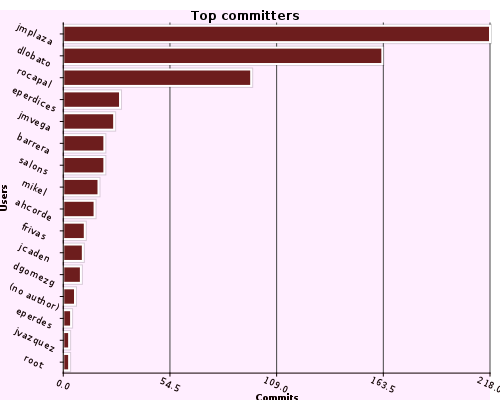
\includegraphics[width=7cm]{figs/svn_top-committers.png}
\caption{Top committers of Jderobot project}
\label{fig:svn-topcommiters}
\end{figure}

Some long term students have contributed continuously for several years, as can be seen at Figure \ref{fig:svn-topcommiters}. They have formed a stable developer core group of 4 or 5 people, all of them in a volunteer basis. In the last years, instead of having a reduced team of developers, we have opened the write access on Jderobot repository to relatively new users. Due to the large software size and the high rotation in the small developer team this has been very beneficial. The maintenance of the framework has already started to be more distributed.

\begin{figure}
  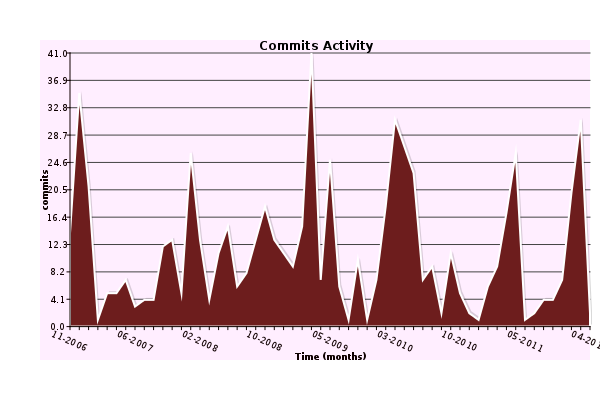
\includegraphics[width=7cm]{figs/svn_activity.png}
\caption{Activity of commits in the project}
\label{fig:svn-activity}
\end{figure}

Figure \ref{fig:svn-activity} shows the activity of software improvement as number of commits in the official repository. The high activity peaks are related with the release of a new Jderobot revision and its debugging period.

\section{Conclusions}

%what have we presented in this paper
We have presented the Jderobot open-source framework for developing robotic applications and research. This is a long term effort with ten years of experience. It provides several drivers for accessing different sensors, robots and actuators like kinect, Nao humanoid, Pioneer robot, cameras, pantilt units, etc.. It also includes a powerful set of tools and libraries that speed up the creation of new robotic applications, like one for visual programming of hierarchical FSM, one for camera calibration, record of log files with sensor data and replay them, viewers and teleoperators, etc. Several successful applications and research developed using the framework have been also presented as experimental validation of its usefulness.

%balance of design principles
The framework's main software architecture principle is the modular design of applications in concurrent components that interact among them through explicit standard interfaces. Each component is a software process, maybe with several threads, with a target. This modular design has proben to be easier to maintain and expand than previous monolithic and centralized releases of the framework. Only components relevant for a given application needs to be installed and new functionality may appear as new components.

The standard interfaces have proben very advantageous for research. For instance, the same localization algorithm can be tested seemlessly with the real cameras, simulated ones, images from a video or from a log file as these image sources strictly follow the same interface. The portability between different robot platforms are also favored by standard interfaces. For example, experiments with the visual memory research component have been performed both in a wheeled Pioneer robot and a humanoid Nao robot without changing the source code, just providing the different robot geometry through configuration files, taking benefit of the same interfaces offered in both robot platforms.
% (camera, pose3Dencoders, pose3Dmotors and encoders)

The use of communication middleware like ICE provides Jderobot with multiplatform and multilanguage support, as components can be writen in C, C++, Java, Python, etc.. It also provides with distribution as the components can run in the same machine or different ones, even with different operating systems. For instance, a teleoperator has been presented with a component running in a smartphone interacting with the NaoServer in the Linux computer onboard the humanoid robot. Another advantage of using ICE is that we haven't taken much care of communications, focusing our efforts on robotics aspects of the components.

Iterative execution of components is recommended in Jderobot and it has proben good for reactive controllers, Bayesian estimators, localization algorithms or image processing applications. In addition, the programming of component GUI in a separate thread and its optional nature are also suggested, and they have shown to be advantageous as fully decouple the processing from the visualization, which can be switched on and off at run time at will without disturbing the robotic processing.

The intensive use of open-source tools and libraries has shown to be a good decision. They have allowed us to reach interesting functionality and results with a reduced set of developers, because we lie as much as possible on existing open-source community software like PCL, Gazebo, Opencv, OpenGL, GSL, etc. Software sharing speeds up and widen the project development. This belief has also motivated us to open the source code of Jderobot.

Two Jderobot's tools, the recorder and replayer components, are very useful in research. They allow, for instance, the fair comparison of different localization algorithms with exactly the same input data, those stored in the log file. A MonteCarlo localization algorithm has been so compared to our evolutive localization algorithm. In the same way, using our CameraServer from filed images our MonoSLAM algorithm have been tested with the same video images as the original Davison's MonoSLAM algorithm.

% more lessons 
We think Jderobot already has reached a good level of software reuse, but mainly for hardware abstraction layer. The same driver components and basic interfaces to access sensors and robots are used in different applications. This software reuse has not scaled yet to more complex robot functionality, maybe because the behavior abstraction is more slippery than traditional function invokation. We are working on this, focusing on reusable localization and local navigation components. The Jderobot tools have also been reused in different scenarios. For instance, the same calibration tool has been used to calibrate the cameras in ElderCare application, for the Nao humanoid camera or for the simulated cameras in Gazebo in the robotics course.

The developer team under Jderobot is small and with high rotation. One lesson learnt is that opening Jderobot development to several students, even new ones, is beneficial. Typical contribution is that of a new student becoming responsible of a single component, its development or updating. The modular design of Jderobot makes it possible. Another good decision has been to recommend our students that their applications should work always with the latest Jderobot release at the repository. This way bugs are solved in the official repository for everyone, everybody take benefit of their solution and there are no several co-existing branches at the same time.

The creation of debian packages made easier the use of the platform in teaching, for newbie users that don't have time to fully learn the whole platforms in two weeks. In addition the specific IntroRob component hides some of the platform complexity, and so the students take shorter time to start using jderobot. The platform is just an instrument to learn robotics, not the goal.

%why not using ROS?
The use of communication middleware like ICE has allowed the programming of Jderobot components in smartphones easily interacting with other components in laptop or personal computers. This flexibility is a key difference between Jderobot and ROS. 

ROS set of drivers is larger than ours.

Tiene ROS un replay-recorder?.

%future lines
- Improved use of ICE advanced capabilities like Icestorm and Icebox.
- Wrappers to use drivers from other platforms wider than ours.

\begin{acknowledgements}
This work has been supported by the project S2009/DPI-1559, RoboCity2030-II, from the Comunidad de Madrid and by the project 10/02567 from the Spanish Ministry of Science and Innovation. Authors want also to thank the contribution to Jderobot project to all developers, in particular Alejandro Hernández and Maikel González.
\end{acknowledgements}

% BibTeX users please use one of
\bibliographystyle{spbasic}      % basic style, author-year citations
%\bibliographystyle{spmpsci}      % mathematics and physical sciences
%\bibliographystyle{spphys}       % APS-like style for physics
\bibliography{bibliografia}   % name your BibTeX data base


\end{document}


